\documentclass{article}
\usepackage{graphicx}
% If you're new to LaTeX, here's some short tutorials:
% https://www.overleaf.com/learn/latex/Learn_LaTeX_in_30_minutes
% https://en.wikibooks.org/wiki/LaTeX/Basics

% Formatting
\usepackage[utf8]{inputenc}
\usepackage[margin=1in]{geometry}
\usepackage[titletoc,title]{appendix}

% Math
% https://www.overleaf.com/learn/latex/Mathematical_expressions
% https://en.wikibooks.org/wiki/LaTeX/Mathematics
\usepackage{amsmath,amsfonts,amssymb,mathtools}
\usepackage{bm}
\usepackage{siunitx}

% Images
% https://www.overleaf.com/learn/latex/Inserting_Images
% https://en.wikibooks.org/wiki/LaTeX/Floats,_Figures_and_Captions
\usepackage{graphicx,float}

% Tables
% https://www.overleaf.com/learn/latex/Tables
% https://en.wikibooks.org/wiki/LaTeX/Tables

% Algorithms
% https://www.overleaf.com/learn/latex/algorithms
% https://en.wikibooks.org/wiki/LaTeX/Algorithms
\usepackage[ruled,vlined]{algorithm2e}
\usepackage{algorithmic}

% Code syntax highlighting
% https://www.overleaf.com/learn/latex/Code_Highlighting_with_minted
\usepackage{minted}
\usemintedstyle{borland}

% References
% https://www.overleaf.com/learn/latex/Bibliography_management_in_LaTeX
% https://en.wikibooks.org/wiki/LaTeX/Bibliography_Management
\usepackage{biblatex}
\addbibresource{references.bib}

\DeclareMathOperator{\taninv}{tan\,inverse}

% Title content
\title{ENPM 673 Homework 1}
\author{Arjun Srinivasan Ambalam, Praveen Menaka Sekar, Arun Kumar Dhandayuthabani}
\begin{document}

\maketitle

% Introduction and Overview
\section{Problem 1}
Assume that you have a camera with a resolution of 5MP where the camera sensor is square shaped with a width of 14mm. It is also given that the focal length of the camera is 15mm.
\begin{itemize}
\item Compute the Field of View of the camera in the horizontal and vertical direction. [10 POINTS]
\item Assuming you are detecting a square shaped object with width 5cm, placed at a distance of 20 meters from the camera, compute the minimum number of pixels that the object will occupy in the image. [10 POINTS]
\end{itemize}
% Example Subsection
\subsection{Field of View Calculation}
Since camera sensor is square shaped and also a single focal length is given,the Field of View (FOV) in Horizontal and Vertical directions are same.
%\boldmath
\begin{equation}
\boxed{FOV =\ 2*\phi} \\
\end{equation}
\begin{equation}
\boxed{\phi = \ \tan ^{-1} \frac{d}{2f}}
\end{equation}
\begin{align*}
\phi =& \ \tan ^{ - 1}\frac{14}{2*15} \\
\phi =& \ \ang{25.0168}\\
FOV =& \ 2*25.0168 \\ =& \ \ang{50.036}
\end{align*}
%\unboldmath
where 
\begin{itemize}
\item d is camera sensor width (d=14 mm)
\item f is focal length (f=15 mm)
\end{itemize}
Therefore the Field of View of the camera (FOV) in horizontal and vertical direction is \boxed{\ang{50.036}}

% Example Subsubsection
\subsection{Minimum number of pixels occupying image}
Given:
\begin{itemize}
    \item Width of square shaped object (w) = 50 mm (5 cm)
    \item Distance of square shaped object from the camera (D) = 20000 mm (20 m)
\end{itemize}
Let the size of object in the image be 'x' mm. Then, 
\begin{equation}
\boxed{\frac{x}{2f}=\frac{w}{2D}}
\end{equation}
After substitution and solving we get,
\begin{equation}
\boxed{x = 0.0375 \ mm}
\end{equation}
\begin{equation}
5 \ MP \ resolution \ for \ sensor area = 14\times14\hspace{.1cm}mm ^2 \\
\end{equation}
\begin{equation}
For \ sensor \ area \ 0.0375\times0.0375\hspace{.1cm}mm ^2 = 35.87 pixels \\
\end{equation}
Therefor minimum number of pixels occupying image is \boxed{35.87}

\section{Problem 2}
Two files of 2D data points are provided in the form of CSV files (Dataset1 and Dataset2). The data represents measurements of a projectile with different noise levels. Assuming that the projectile follows the equation of a parabola,
\begin{itemize}
    \item Find the best method to fit a curve to the given data for each case. You have to plot the data and your best fit curve for each case. Submit your code along with the instructions to run it. [40 POINTS]
    \item Briefly explain all the steps of your solution and discuss why your choice of outlier rejection technique is best for that case. [20 POINTS]
\end{itemize}
\subsection{Curve Fitting}
The problem of curve fitting is, given N discrete points in space, to find model parameters that can best characterize or generalize the trends prevailing between them. For this assignment, we are given with a set of 2D data points representing a projectile with different noise levels. In order to obtain the best model that can fit the given data points, We have discussed about Least Squares, Total Least Squares, Least Squares with Regularization and RANSAC (Random Sample Consensus) methodologies. Based on the results obtained from the above methods, the best fit for the problem is decided. Let us have a brief look at each of the above methods and their corresponding results.
\newline \newline \textbf{Least Squares:}
\newline Given the 2D projectile data \{(X\textsubscript{1}, Y\textsubscript{1}), (X\textsubscript{2}, Y\textsubscript{2}), ......., ( X\textsubscript{N}, Y\textsubscript{N})\}, we try to fit a quadratic equation $y = a{x^2} + bx + c$ by reducing the sum of squared errors associated with the estimated model parameters and ground truth. This concept is mathematically represented by,
\begin{equation}
\boxed{E(a, b, c) = \sum_{n = 1}^{N} (y - (a{x^2} + bx + c))}
\end{equation}
where,
\begin{itemize}
    \item E(a, b, c) - sum of squared errors between the ground truth y and the estimate y obtained from our model parameters. 
\end{itemize}
In order to find best fit for the above data we try to minimize the above error with respect to the model parameters. This can be easily represented using matrices.
\begin{equation}
\boxed{Y = XB}
\end{equation}
where, 
\begin{equation}
\boxed{Y = 
\begin{bmatrix}
y_1 \\ y_2 \\ . \\ . \\ . \\ y_N
\end{bmatrix}
X = 
\begin{bmatrix}
x^2_1 & x_1 & 1 \\ x^2_2 & x_2 & 1 \\ . & . & . \\ . & . & . \\
x^2_N & x_N & 1 
\end{bmatrix}
B = 
\begin{bmatrix}
a \\ b \\ c
\end{bmatrix}}
\end{equation}
\begin{equation}
\boxed{E(a, b, c) = (Y - XB)^2}
\end{equation}
In order to minimize the above error,
\begin{equation}
\boxed{\frac{\partial E(a, b, c)}{\partial B} = 0}
\end{equation}
On solving the above equation we obtain the following optimized model parameters,
\begin{equation}
\boxed{B = (X^TX)\textsuperscript{-1}(X^TY)}
\end{equation}
\begin{algorithm}
\SetAlgoLined
\KwResult{Y\textsubscript{estimate}}
 Load 2D data points\;
 Evaluate Y and X matrices\;
 Evaluate B matrix from $B = (X^TX)\textsuperscript{-1}(X^TY)$\;
 Evaluate and Return Y\textsubscript{estimate}\;
 Scatterplot original 2D data points and Plot the curve that fit the 2D
 data points
\caption{LeastSquaresCurveFitting.py}
\end{algorithm}

\begin{center}
    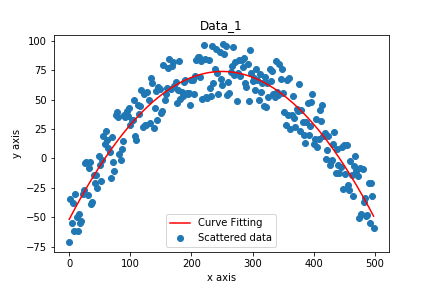
\includegraphics{least_square_curvefitting_data_1.png}
    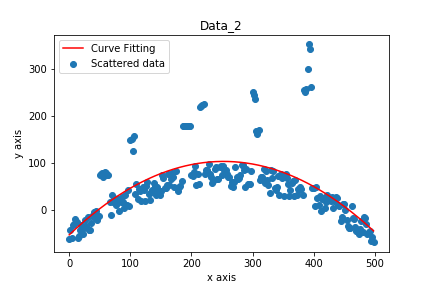
\includegraphics{least_square_curvefitting_data_2.png}
\end{center}

\newline \newline \textbf{Least Squares with Regularization:}
\newline Given the 2D projectile data \{(X\textsubscript{1}, Y\textsubscript{1}), (X\textsubscript{2}, Y\textsubscript{2}), ......., ( X\textsubscript{N}, Y\textsubscript{N})\}, we try to fit a quadratic equation $y = a{x^2} + bx + c$ by reducing the sum of squared errors associated with the estimated model parameters and ground truth with an addition constraint called regularization parameter. This concept is mathematically represented by,
\begin{equation}
\boxed{E(a, b, c) = \sum_{n = 1}^{N} (y - (a{x^2} + bx + c))}
\end{equation}
where,
\begin{itemize}
    \item E(a, b, c) - sum of squared errors between the ground truth y and the estimate y obtained from our model parameters. 
\end{itemize}
In order to find best fit for the above data we try to minimize the above error with respect to the model parameters. This can be easily represented using matrices.
\begin{equation}
\boxed{Y = XB}
\end{equation}
where, 
\begin{equation}
\boxed{Y = 
\begin{bmatrix}
y_1 \\ y_2 \\ . \\ . \\ . \\ y_N
\end{bmatrix}
X = 
\begin{bmatrix}
x^2_1 & x_1 & 1 \\ x^2_2 & x_2 & 1 \\ . & . & . \\ . & . & . \\
x^2_N & x_N & 1 
\end{bmatrix}
B = 
\begin{bmatrix}
a \\ b \\ c
\end{bmatrix}}
\end{equation}
\begin{equation}
\boxed{E(a, b, c) = (Y - XB)^2}
\end{equation}
In order to minimize the above error,
\begin{equation}
\boxed{\frac{\partial E(a, b, c)}{\partial B} = 0}
\end{equation}
On solving the above equation we obtain the following optimized model parameters,
\begin{equation}
\boxed{B = (X^TX)\textsuperscript{-1}(X^TY)}
\end{equation}
\begin{center}
    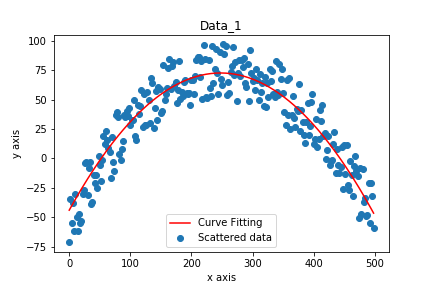
\includegraphics{least_square_regularization_data_1.png}
    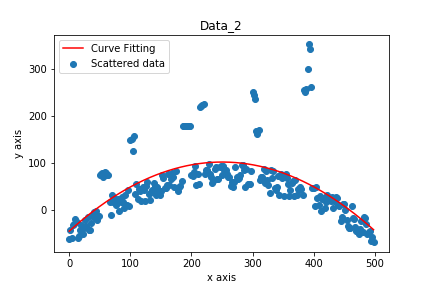
\includegraphics{least_square_regularization_data_2.png}
\end{center}

\newline \textbf{Random Sample And Consensus (RANSAC)}:
\newline
RANSAC is an iterative algorithm that estimates the best possible solution of a certain model using the given set of data points that is contaminated by large number of outliers. RANSAC basically comprises of two steps:
\begin{itemize}
    \item Minimal Sample Sets were randomly selected from the input dataset (for a quadratic curve minimum number of points required and the model parameters are computed using only those elements; in order to compute model parameters we can use least squares or total least squares or any other optimization methodologies.
    \item We then evaluate the model estimated by checking it with rest of the dataset and classify the dataset into inliers and outliers based on a defined threshold.
\end{itemize}
\begin{algorithm}[H]
\SetAlgoLined
\KwResult{Best Model Parameters}
 Obtain minimum number of samples, minimum number of inlier points, threshold, iterations\;
 Initialize best model = None, best inliers = 0, best error = infinity, i = 0\;
 \While{i $\leq$ iterations}{
  Choose 3 random points from the dataset\;
  Also obtain the remaining points from the dataset\;
  Fit a curve for the 3 random points using least squares method\;
  Estimate the y values for the remaining points\;
  Find the error per point\;
  Compute the number of inliers by comparing the error per point with threshold\;
  \If{number of inliers $\geq$ minimum number of inlier points}{
   Total number of inliers = number of inliers + minimum number of samples\;
   Fit a curve again for the set containing Total number of inliers\;
   Estimate the y values for the remaining points\;
   Find the error per point and calculate the mean of the error\;
   \If{current error $\leq$ best error}{
   best model = current model\;
   best error = current error\;
   best inliers = total inliers\;
   }
      }
      i = i + 1\;
 }
 \caption{Random Sample And Consensus (RANSAC)}
\end{algorithm}
\begin{center}
    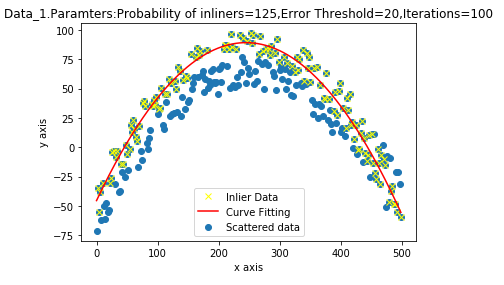
\includegraphics{Data_1_Parameter_1.png}
    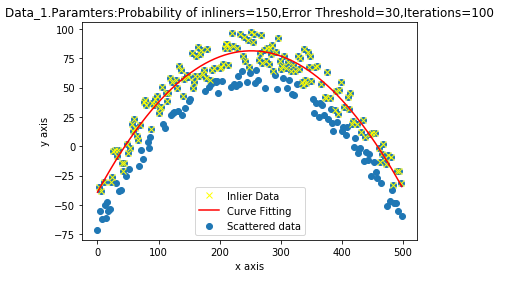
\includegraphics{Data_1_Parameter_2.PNG}
    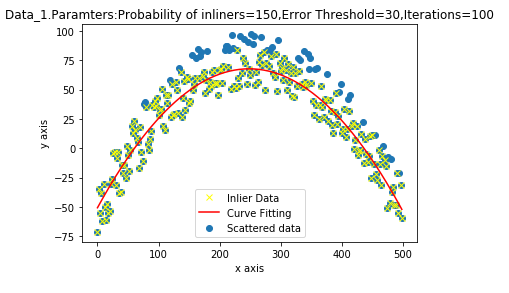
\includegraphics{Data_1_Paramter_3.png}
    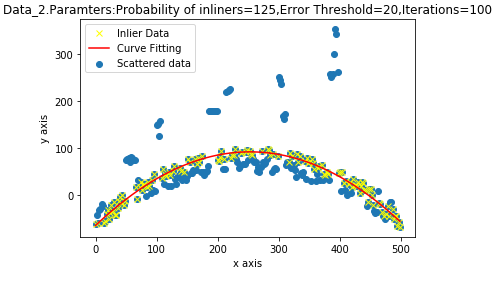
\includegraphics{Data_2_Parameter_1.PNG}
    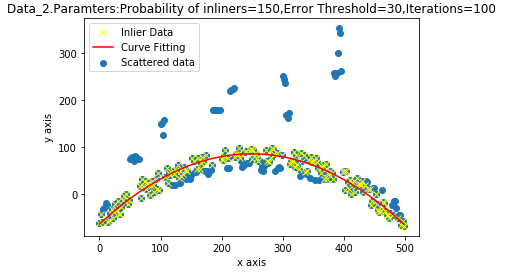
\includegraphics{Data_2_Parameter_2.PNG}
    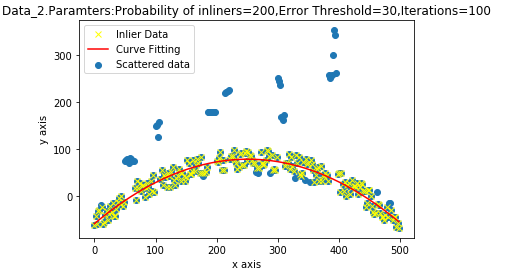
\includegraphics{Data_2_Parameter_3.PNG}
\end{center}
\\
\\
\vspace{40mm} %5mm vertical space
\section{Homography in Computer Vision}

\begin{flushleft}


\begin{equation*}
A = 
\begin{bmatrix}
-x1 & -y1 & -1 & 0 & 0 & 0 & x1*xp1 & y1*xp1 & xp1 \\
 0 & 0 & 0 & -x1 & -y1 & -1 & x1*yp1 & y1*yp1 &yp1 \\
-x2 & -y2 & -1 & 0 & 0 & 0 & x2*xp2 & y2*xp2 & xp2 \\
 0 & 0 & 0 & -x2 & -y2 & -1 & x2*yp2 & y2*yp2 &yp2 \\
-x3 & -y3 & -1 & 0 & 0 & 0 & x3*xp3 & y3*xp3 & xp3 \\
 0 & 0 & 0 & -x3 & -y3 & -1 & x3*yp3 & y3*yp3 &yp3 \\
-x4 & -y4 & -1 & 0 & 0 & 0 & x4*xp4 & y4*xp4 & xp4 \\
 0 & 0 & 0 & -x4 & -y4 & -1 & x4*yp4 & y4*yp4 &yp4 
\end{bmatrix}
\end{equation*}



where,

\begin{center}
\begin{tabular}{ |c|c|c|c|c|c| } 
\hline
index & x & y & xp & yp \\
\hline
\multirow
1 & 5 & 5 & 100 & 100 \\ 
2 & 150 & 5 & 200 & 80 \\
3 & 150 & 150 & 220 & 80 \\
4 & 5 & 150 & 100 & 200 \\
\hline
\end{tabular}
\end{center}

Substituting the values, the A matrix becomes

\begin{equation*}
A = 
\begin{bmatrix}
-5 & -5 & -1 & 0 & 0 & 0 & 500 & 500 & 100 \\
 0 & 0 & 0 & -5 & -5 & -1 & 500 & 500 & 100 \\
-150 & -5 & -1 & 0 & 0 & 0 & 30000 & 1000 & 200 \\
 0 & 0 & 0 & -150 & -5 & -1 & 12000 & 400 & 80 \\
-150 & -150 & -1 & 0 & 0 & 0 & 33000 & 33000 & 220 \\
 0 & 0 & 0 & -150 & -150 & -1 & 12000 & 12000 & 80 \\
-5 & -150 & -1 & 0 & 0 & 0 & 500 & 15000 & 100 \\
 0 & 0 & 0 & -5 & -150 & -1 & 1000 & 30000 & 200 
\end{bmatrix}
\end{equation*}

To compute SVD for Matrix A ,we need to calculate  eigen values and vectors of $A^{\rm T}$A matrix \\
\[ A &= U\Sigma V^{T} \] \\
A is a matrix of size 8\times 9\\
The columns of V (size:9\times 9) are  \ orthogonal \ eigenvectors \ of $A^{\rm T}$A \\
Eigenvalues  of $A^{\rm T}$A  are \lamda 1 … \lambda r \\
\sigma i=\sqrt {\lambda i}\\
\sum_= diag(\sigma 1...\sigma 9)
\vspace{5mm} %5mm vertical space

 
 


\vspace{5mm} %5mm vertical space
V=\begin{bmatrix}
    0.0028  &  0.0031  & -0.2464 &  -0.1586  & -0.1752 &   0.1767 &   0.9137  & -0.1203 &   0.0531\\
    0.0024  & -0.0013  & -0.3770 &   0.1766  &  0.6895 &   0.5903 &  -0.0529  & -0.0022 &  -0.0049\\
    0.0000  &  0.0000  & -0.0024 &  -0.0037  &  0.0052 &   0.0075 &   0.0660  &  0.7860 &   0.6146\\
    0.0011  &  0.0012  &  0.6612 &   0.3412  &  0.5017 &  -0.2325 &   0.3721  & -0.0426 &   0.0177\\
    0.0016  & -0.0029  &  0.5743 &  -0.0710  & -0.3145 &   0.7499 &  -0.0620  &  0.0046 &  -0.0039\\
    0.0000  &  0.0000  &  0.0058 &  -0.0022  &  0.0029 &  -0.0057 &  -0.1225  & -0.6049 &   0.7868\\
   -0.6961  & -0.7180  & -0.0001 &  -0.0038  &  0.0025 &  -0.0002 &   0.0044  & -0.0006 &   0.0002\\
   -0.7180  &  0.6961  &  0.0016 &  -0.0038  &  0.0025 &   0.0037 &  -0.0006  & -0.0000 &   0.0000\\
   -0.0062  &  0.0000  & -0.1735 &   0.9067  & -0.3783 &   0.0622 &   0.0252  & -0.0025 &   0.0076\\

\end{bmatrix}
\vspace{5mm} %5mm vertical space


\sum_= \begin{bmatrix}
 \vspace{5mm} %5mm vertial space

      60214.89 &         0    &     0  &       0   &      0    &     0   &      0     &    0     &    0\\
         0  &     31824.52     &   0   &      0    &     0     &    0    &     0   &      0      &   0 \\
         0   &      0       & 260.89   &      0    &     0     &    0  &       0    &     0      &   0 \\
         0   &      0       &  0    &    186.22    &     0     &    0     &    0    &     0      &   0 \\
         0   &      0       &  0    &     0     &   145.60     &    0      &   0    &     0      &   0 \\
         0   &      0       &  0    &     0     &    0      &   60.87      &   0    &     0      &   0 \\
         0   &      0       &  0    &     0     &    0      &   0       &   3.87    &     0      &   0 \\
         0   &      0       &  0    &     0     &    0      &   0       &  0     &     0.81      &   0 \\
         0   &      0       &  0    &     0     &    0      &   0       &  0     &     0      &   0 \\
\end{bmatrix}\\
\vspace{5mm} %5mm vertical space
Where U matix is obtained by multiplying A and V matrices and dividing the coloums of AV with corresponding \sigma i (i=1 \ to \ 9)
% U_i=(\displaystyle \frac {AV}{\sigma i} )\\

\vspace{5mm} %5mm vertical space
U=\begin{bmatrix}
    -0.0118  & -0.0003 &  -0.0516  & 0.4661  & -0.2603  &  0.0678  &  0.0108 &  -0.8411& 0\\
    -0.0118  &  -0.0003 &   -0.0872 &  0.4594  & -0.2491  & 0.0886  & 0.7655  &  0.3542& 0\\
    -0.3587  &  -0.6549 & 0.0135  & 0.4651  &  0.1701  &  -0.2936  & -0.2784  &  0.1823& 0\\
    -0.1435  &  -0.2620 &   -0.4454 &   -0.1361  & -0.5008 &  0.5875 &  -0.2731 &   0.1529& 0\\
    -0.7750  &  -0.0227 &  0.4085  &  -0.2849 &   0.0320 &  0.2352 &   0.2627  & -0.1597& 0\\
    -0.2818  &  -0.0082 &   -0.6922  &  -0.3159  &  0.0114  &  -0.5019  &  0.2466 &  -0.1696& 0\\
    -0.1846  & 0.3168 &  0.2485 &  0.0347  & -0.6983 &   -0.4673  & -0.2524  &  0.1816& 0\\
    -0.3693  & 0.6336  &  -0.2889  & 0.3933  &  0.3189  & 0.1750 &  -0.2614  &  0.1526& 0\\
\end{bmatrix}\\





\end{flushleft}


\end{document}